%\lstset{basicstyle=\small\ttfamily,
%        emphstyle=\bfseries,
%        columns=fixed,
%        numbers=left,xleftmargin=2em,frame=single,framexleftmargin=1.5em,
%        moredelim=*[l][\textit]{//},
%        moredelim=*[l][\bfseries]{\#},
%        literate={...}{\dots}3
%} 
\subsection{Task-based Programming Models}
\label{sec.background}
\begin{lstlisting}[float, emph={Dependency,DepList,Data}, captionpos=b, caption={Compiler generated pseudo-code equivalence for task annotation.},label=task_clause]
     ...
  //task_clause
  memalloc(&task, args, size);
  createTask(deps, task, parent, taskData);
     ...
\end{lstlisting}
\begin{lstlisting}[float, emph={createTask}, captionpos=b, caption={Pseudo-code for task creation.},label=taskCreation, emph={[2]mat}, emphstyle={[2]}, aboveskip={0\baselineskip}, frame=tb, belowskip={0\baselineskip}]
void createTask(DepList dList, Task t,  
                Task parent, Data args) {
  initAndSetupTask(task1, parent, args);
  insertToTDG(dList, task1);
}
\end{lstlisting}

Task-based parallel programming models ~\cite{Blumofe:PPoPP1995, Reinders2007, Bauer2012, OmpSs},  are widely used to facilitate the programming of parallel codes for multi-core systems.
These programming models offer annotations that the programmer can add to the application's sequential code.
One type of these annotations is the task annotations with dependency tracking which OpenMP~\cite{OpenMP} supports since its 4.0 release~\cite{OpenMP4.0:Manual2015}. 
By adding these annotations, the programmer decomposes the application into \textit{tasks} and specifies the input and output data dependencies between them. 
A compiler is responsible to translate the annotations into code by adding calls to the programming model's runtime system. 
The runtime system consists of software threads and is responsible for the efficient execution of the tasks with respect to the data dependencies as well as the availability of resources.

When the compiler encounters a task annotation in the code, it transforms it to the pseudo-code shown in Listing~\ref{task_clause}.
\texttt{Memalloc} is performing the memory allocation for the task and its arguments.
Next is a runtime call, which is the \texttt{createTask}, responsible for the linking of the task with the runtime system.
At this point a task is considered \textit{created} and below are the three possible states of a task inside the runtime system:
\begin{itemize}
\item \textit{Created:} A task is initialized with the appropriate data and function pointers and it is inserted in the Task Dependency Graph (TDG). The insertion of a task in the TDG implies that the data dependencies of the tasks have been identified and the appropriate data structures have been created and initialized. 
%At this point a task is considered as \textit{created} but not \textit{ready}.
%\item \textit{TDG Submission:} After the allocation, a task is being inserted in the Task Dependency Graph (TDG). The insertion of a task in the TDG implies that the data dependencies of the tasks have been identified and the appropriate data structures have been created and properly initialized. At this point a task is considered as \textit{created} but not \textit{ready}.
\item \textit{Ready:} When all the data dependencies of a created task have been satisfied, the task is ready and it is inserted in the \textit{ready queue} where it waits for execution. 
\item \textit{Finished:} When a task has finished execution and has not been deleted yet.
\end{itemize}

The runtime system creates and manages the software threads for the execution of the tasks. 
Typically one software thread is being bound to each core. 
One of the threads is the \textit{master thread}, and the rest are the \textit{worker threads}. 
The master thread starts executing the code of Listing~\ref{task_clause} sequentially. 
The allocation of the task takes place first.
What follows is the task creation, that includes the analysis of the dependencies of the created task and the connection to the rest of the existing dependencies.
Then, if there are no task dependencies, which means that the task is \textit{ready}, the task is also inserted in the ready queue and waits for execution.
\begin{lstlisting}[float, emph={insertToTDG}, caption={Pseudo-code for TDG insertion},label=insertTDG]
void insertToTDG(DepList dList, Task t) {
  if( dList.isEmpty() ) {
    readyQ$\rightarrow$push(t);
    return;
  }
  Dependency entry;
  for( d in dList ) {
    entry = depMap[d.address()];
    if(entry==NULL) depMap.add(entry, t);
    if(d.accessType() == "write")
      entry.addLastWriter(t);
    if(d.accessType() == "read") {
        entry.addReader(t);
        entry.lastWriter()$\rightarrow$addSuccessor(t);
    }
  }
}
\end{lstlisting}
Listing~\ref{taskCreation} shows the pseudo-code for the task creation step within the runtime.
The \texttt{createTask} function is first initializing the task by copying the corresponding data to the allocated memory as well as connecting the task to its parent task (\texttt{initAndSetupTask}).
After this step, the task is ready to be inserted in the TDG. 
The TDG is a distributed and dynamic graph structure that the runtime uses to keep the information about the current tasks of the application. 
The insertion of a task in the TDG is done by the \texttt{insertToTDG} function.
This function takes as arguments a list with all the memory addresses that are to be written or read by the task (\texttt{dList}), and the task itself.
Listing~\ref{insertTDG} shows the pseudo-code for the TDG insertion. 
If for a task the \texttt{dList} is empty (line 2), this means that there are no memory addresses that need to be tracked during the execution; thus, the task is marked as \textit{ready} by pushing it to the \textit{ready queue} (line 3).
Each entry of \texttt{dList} contains the actual memory address as well as the access type (read, write or read-write).
The runtime keeps a distributed unified dependency tracking structure, the \texttt{depMap} where it stores all the tracked memory addresses together with their writer and reader tasks.
For each item in the \texttt{dList} the runtime checks if there is an existing representation inside the \texttt{depMap} (line 8).
If the memory address of an entry of the \texttt{dList} is not represented in the \texttt{depMap}, it is being added as shown in line 9.
If the address of a \texttt{dList} item exists in the \texttt{depMap}, this means that a prior task has already referred to this memory location, exhibiting a data dependency.
According to the access type of \texttt{d}, the readers and the writers of the specific address are updated in the \texttt{depMap} (lines 10-15).

To reduce the lookup into the \texttt{depMap} calls, every time the contents of a memory address are modified, the tasks keep track of their \textit{successors} as well as the number of \textit{predecessors}.
The \textit{successors} of a task are all the tasks with inputs depending on the output of the current task.
The \textit{predecessors} of a task are the tasks whose output is used as input for the current task.
When a \texttt{read} access is identified, the task that is being created is added to the list of successors of the last writer task, as shown on line 20 of Listing~\ref{taskCreation}.

\begin{lstlisting}[float, emph={task_finish}, caption={Pseudo-code for task$\_$finish runtime activity.},label=taskFinish]
void task_finish(Task *t) {
  depMap.removeReaderWriter(t);
  if(t$\rightarrow$successors.empty()) delete t;
  else {
    for( succ in t$\rightarrow$successors ) {
        succ.decreasePredecessors();
        if(succ.numPredecessors == 0) 
            readyQ$\rightarrow$push(succ);
    }
  }
}
\end{lstlisting}

As tasks are executed, the dependencies between them and their successors are satisfied. 
So the successor tasks that are waiting for input, eventually become \textit{ready} and are inserted to the ready queue.
When a task goes to the \textit{finished} state, the runtime has to perform some actions in order to prepare the successor tasks for execution.
These actions are described in Listing~\ref{taskFinish}.
The runtime first updates the \texttt{depMap} to remove the possible references of the task as reader or writer (line 2).
Then, if the task does not have any successors, it can safely be deleted (line 3).
If the task has successors, the runtime traverses the successor list and for each successor task it decreases its predecessor counter (lines 5-6).
If for a successor task its predecessor counter reaches zero, then this task becomes \textit{ready} and it is inserted in the \textit{ready queue} (lines 7-8).

The runtime activity takes place at the task state changes. 
One state change corresponds to the task creation, so a task from being just allocated it becomes \textit{created}. 
At this point the runtime prepares all the appropriate task and dependency tracking data structures as well as inserts the task into the TDG.
The second change occurs when a task from being \textit{created} it becomes \textit{ready};
this implies that the input dependencies of this task are satisfied so the runtime schedules and inserts the task into the ready queue.
The third change occurs when a running task finishes execution. 
In this case, following our task states, the task from being \textit{ready} it becomes \textit{finished}; this is followed by the runtime updating the dependency tracking data structures and scheduling possible successor tasks that become ready. 
For the rest of the paper we will refer to the first state change runtime activity as the task creation overheads (\textit{Create}).
For the runtime activity that takes place for the following two state changes (and includes scheduling and dependence analysis) we will use the term runtime overheads (\textit{Runtime}).



%\begin{lstlisting}[float, emph={void,if,return,not,true,and,break}, captionpos=b, caption={Pseudo-code for task creation.},label=taskCreation, emph={[2]mat}, emphstyle={[2]}, aboveskip={0\baselineskip}, frame=tb, belowskip={0\baselineskip}]
%
%void createTask(Deplist dList, Task task1, 
%            Task parent, Data taskData) {
%  initAndSetupTask(task1, parent, taskData);
%  insertToTDG(dList, task1);
%}
%
%Dependency depMap[];
%
%void insertToTDG(DepList dList, Task task1) {
% if( dList.empty() ) {
%   rQueue_submission(task1);
%   return;
% }
% Dependency entry;
% for( d in dList ) {
%   entry = depMap.lookupAddress(d.address());
%   if(entry == NULL) 
%     depMap.add(d.address(), d.accessType(), task1);
%   if(d.accessType() == "write") {
%     entry.addLastWriter(task1);
%   }
%   else if(d.accessType() == "read") {
%     entry.addReader(task1);
%     entry.lastWriter()->addSuccessor(task1);
%   }
%   else if(d.accessType() == "read-write") {
%     entry.addLastWriter(task1);
%     entry.addReader(task1);
%   }
%
% }
%}
%\end{lstlisting}


\if 0
\begin{lstlisting}[float, emph={void,if,return,Dependency,DepList,Data,not,true,and,break}, captionpos=b, caption={Pseudo-code for the SRT loop.},label=SRTloop, emph={[2]mat}, emphstyle={[2]}, aboveskip={0\baselineskip}, frame=tb, belowskip={0\baselineskip}]

void TDG_submission(Task *task, Data *dependencies) {
 list tmpDeps;
 for( d in dependencies ) {
   if(d.address() == NULL) continue;
   for( t in tmpDeps ) {
     if(t.address() == d.address()) {
       t.setInput(d.isInput() || t.isInput());
       t.setOutput(d.isOutput() || t.isOutput());
       found = true;
       break;
     }
   }
   if(!found) t.push(d); 
 }
 for( t in tmpDeps ) {
   address=t.address();
   TrackableObject existing = depsMap.lookup(address);
   if( t.type == input ) 
     addDep(t, address, input);
   
 }
 
 return;
}
\end{lstlisting}
\fi

\if 0
\begin{lstlisting}[float, emph={void,if,return,rQueue_submission, not,true,and,break}, captionpos=b, caption={Pseudo-code of the task$_$finish runtime activity.},label=task_finish, emph={[2]mat}, emphstyle={[2]}, aboveskip={0\baselineskip}, frame=tb, belowskip={0\baselineskip}]

task_finish:
  if(numDeps == 0) delete task;
  for( succ in task->successors ) {
    succ.deletePredecessor(task);
    succ.decreasePredecessors();
  	if(succ.numPredecessors == 0) rQueue_submission(succ);
  }
\end{lstlisting}
\fi
\subsection{Motivation}

%\begin{figure}[t!]%
%	\centering
%	\subfigure[Figure 1]{\label{fig:sub1}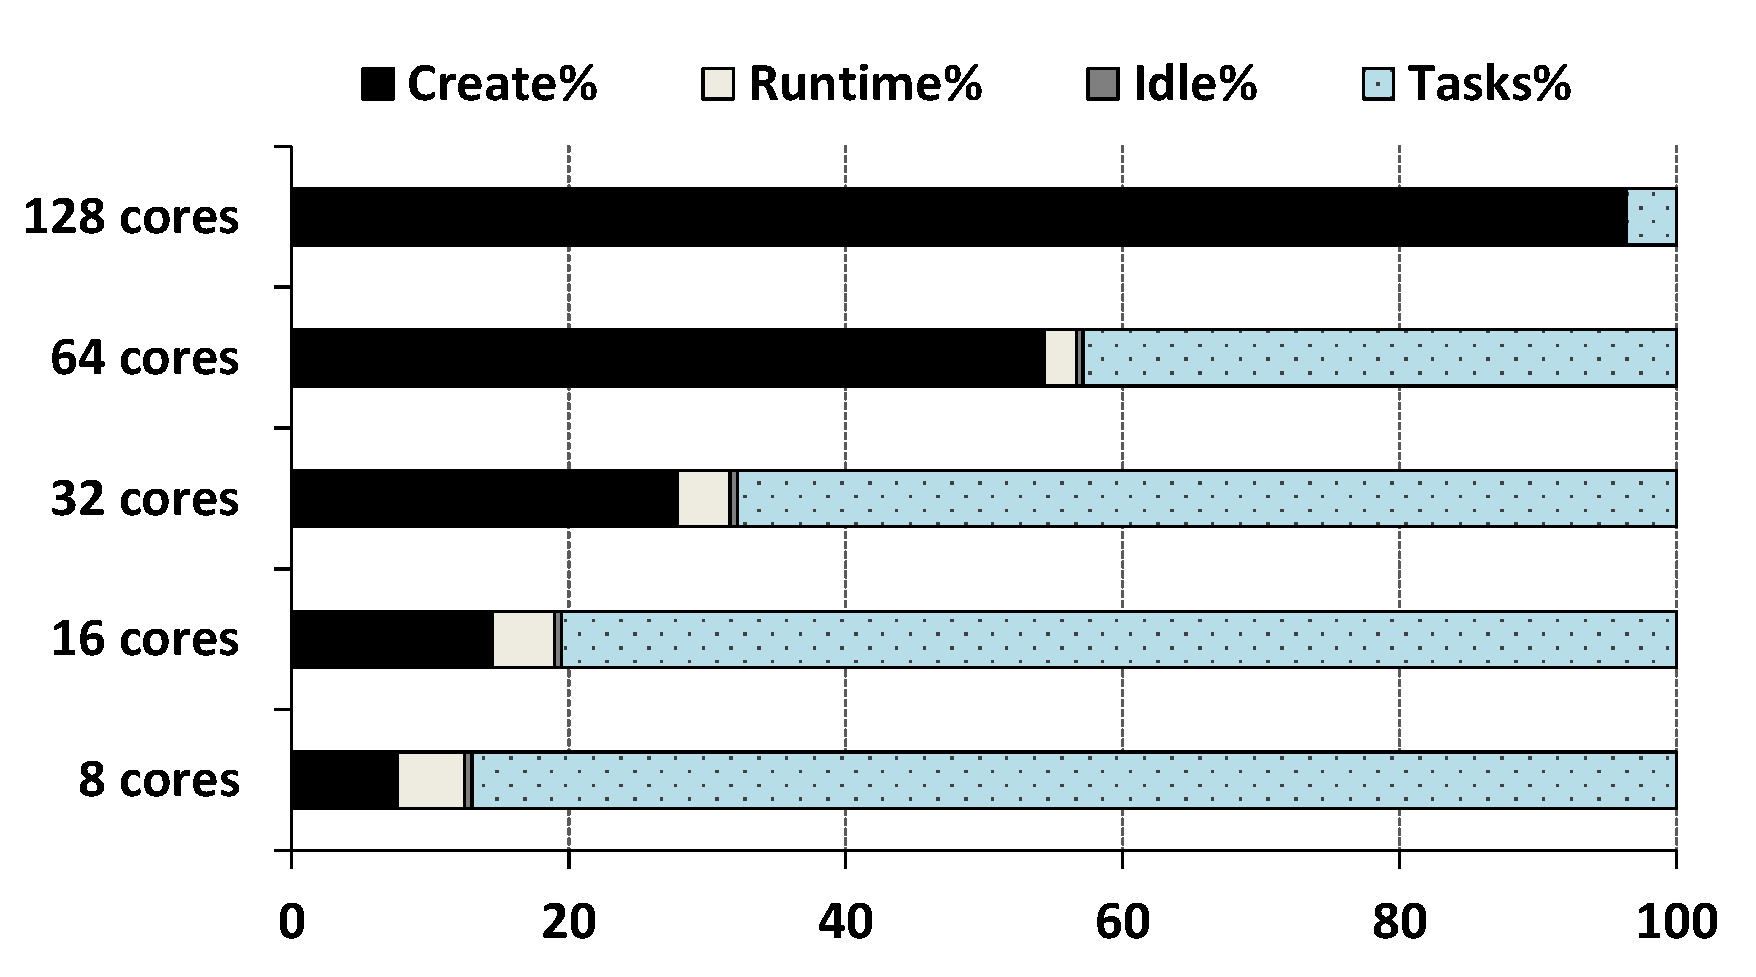
\includegraphics[width=.45\linewidth]{figures/master_thread.pdf}}
%	\subfigure[Figure 1]{\label{fig:sub1}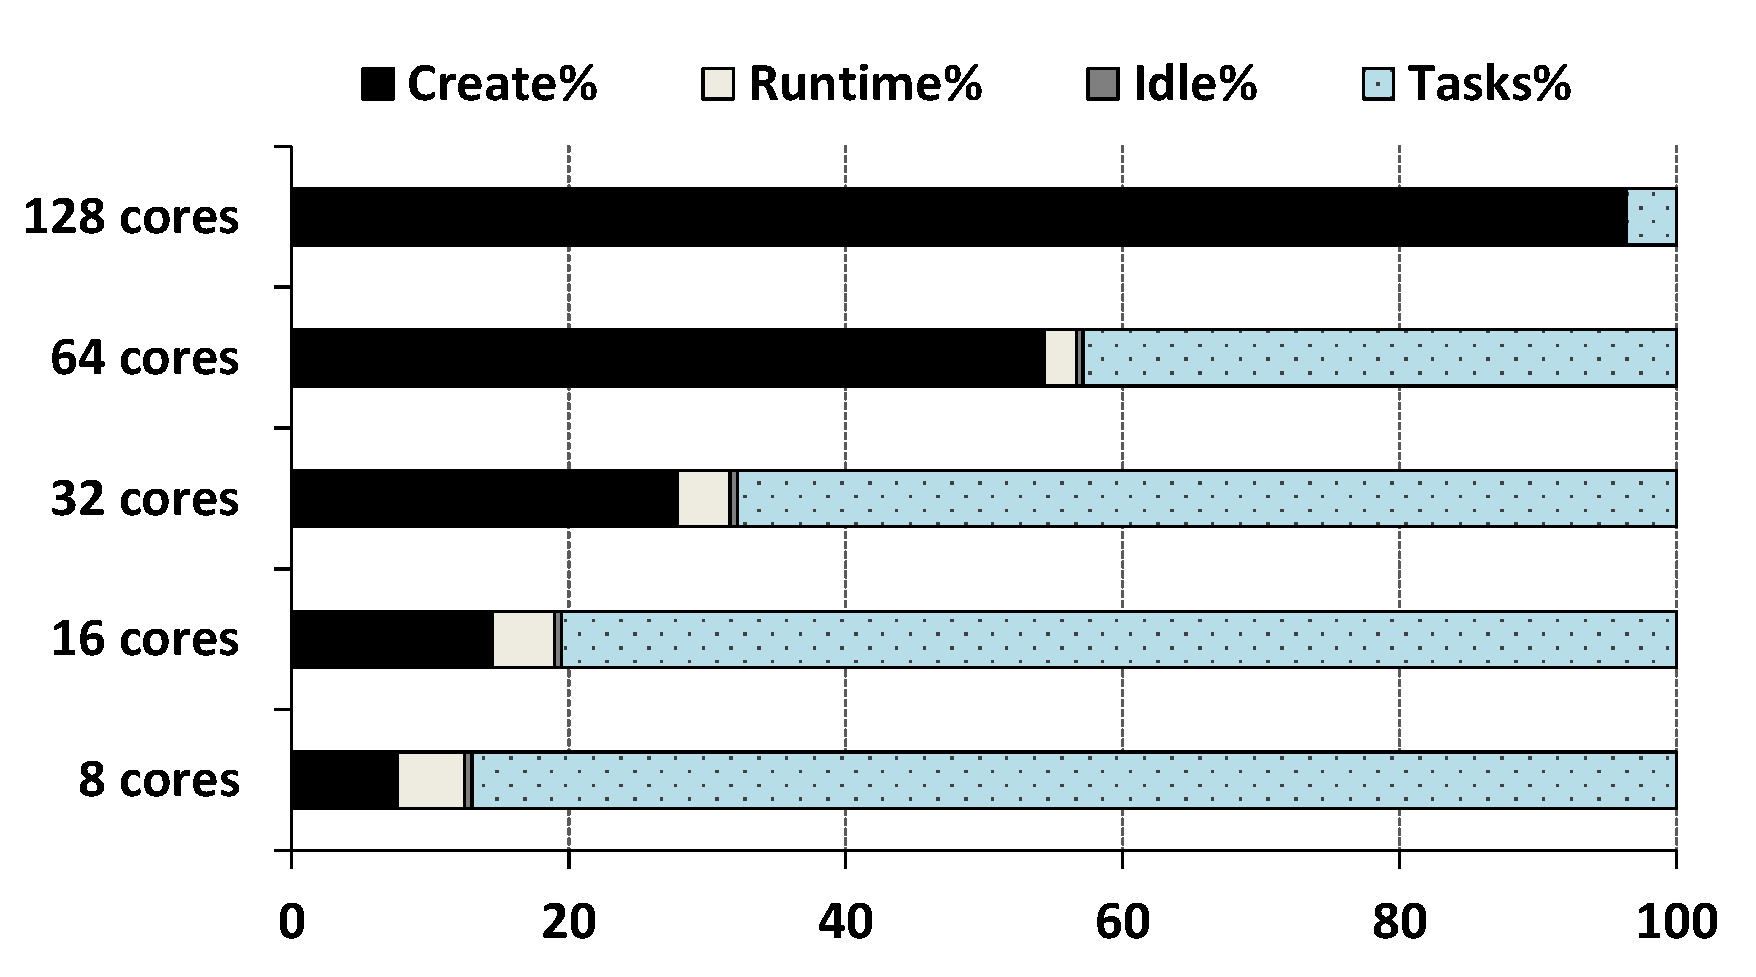
\includegraphics[width=.45\linewidth]{figures/master_thread.pdf}}
%	\caption{My caption}
%\end{figure}


\begin{figure}[t!]%
	\centering
	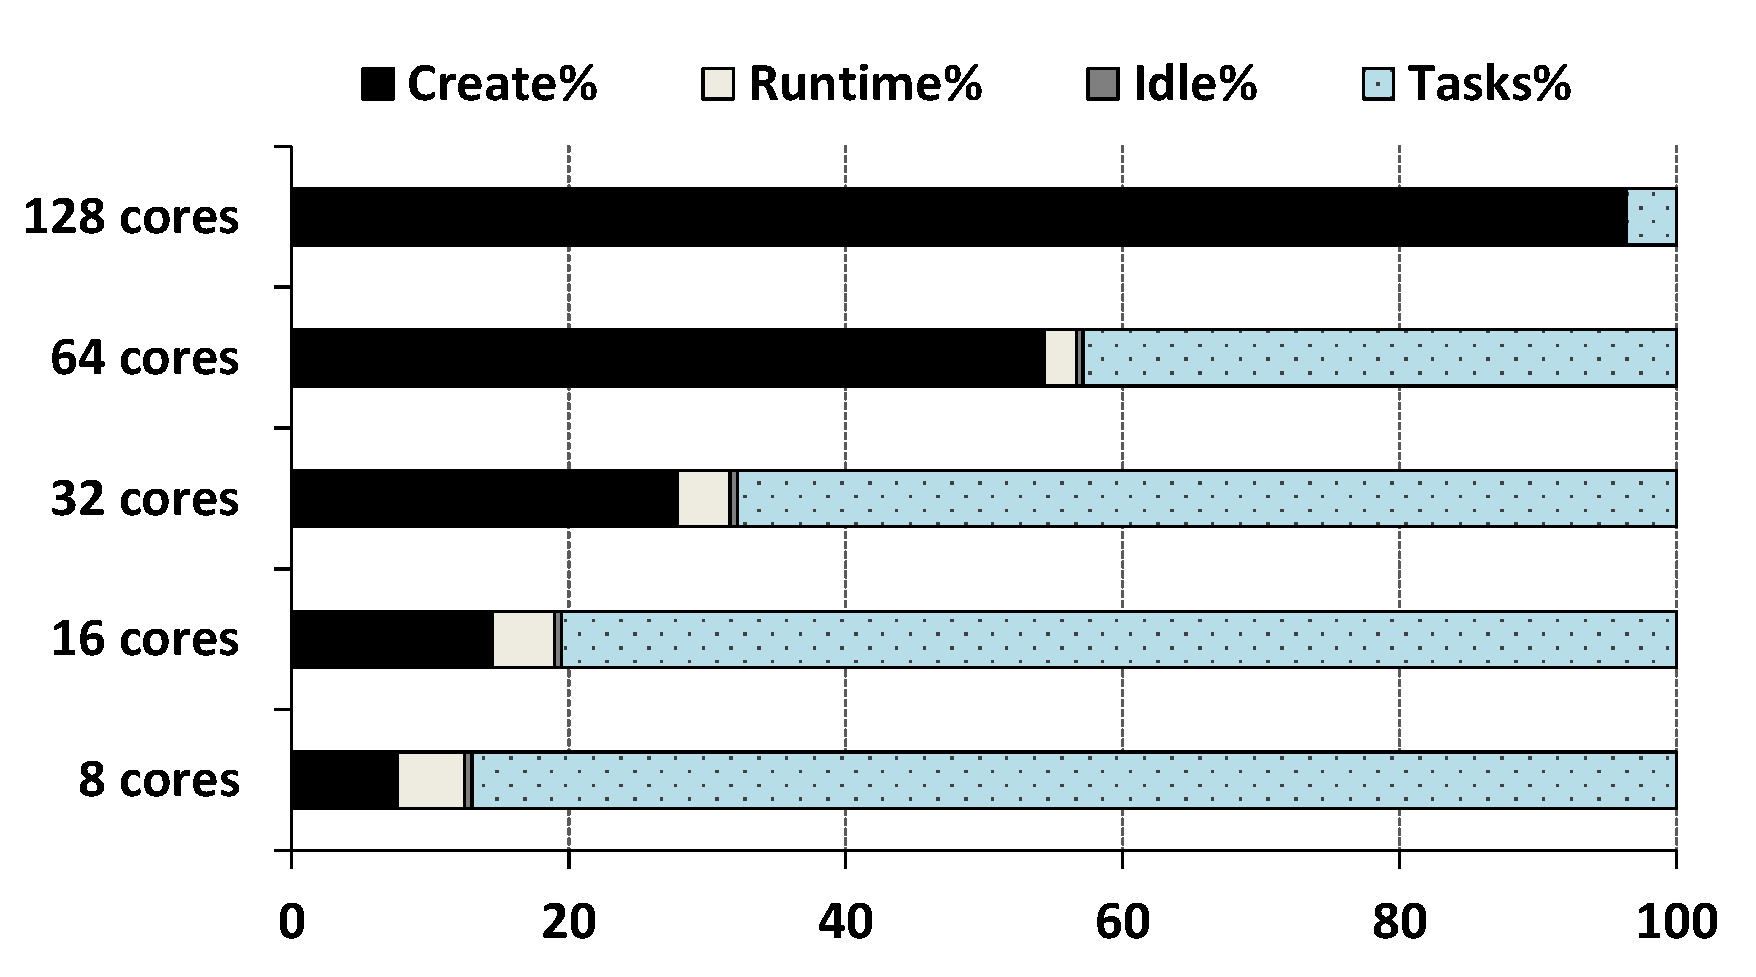
\includegraphics[width=0.75\columnwidth]{figures/master_thread.pdf}
	\caption{Master thread activity for Cholesky as we increase the number of cores.}
	%\caption{Performance improvements on a big.LITTLE processor with different $(F,N)$ configurations, where $F$ is the total number of big cores and $N$ the total number of cores. Results are normalized to running on four little cores with pinned Pthreads.}%
	\label{fig:master_thread}%
\end{figure}

Figure~\ref{fig:master_thread} shows the runtime activity of the master thread during the execution of the Cholesky{\footnote{Details about the benchmarks used are in Section~\ref{sec.background.applications}} benchmark on 8, 16, 32, 64 and 128 cores\footnote{The experimental set-up is explained in Section~\ref{sec.background.arm}}.
The execution time represented here is the wall clock time during the parallel region of the benchmark.
Each one of the series represents a different runtime overhead from the ones described above.
%\textit{Create} represents the \textit{Creation} step, 
%\textit{Runtime} refers to the \textit{Finish} step, \textit{Idle} shows the master thread's idle time and the \textit{Tasks} is the time spent on task execution. 
The percentage of time spent on task creation is increasing as we increase the number of cores.
This is because the creation overhead is invariant of core count: the more we reduce the application's execution time by adding resources the more important this step becomes in terms of execution time.
In contrast, the task execution time percentage is decreased as we increase the number of cores because the computational activity is being shared among more resources.
One way to reduce the task creation overhead is by introducing nested parallelism. 
In this programming technique, every worker thread is able to generate tasks thus the task creation is spread among cores and its overhead is reduced.
However, not all applications can be implemented with this parallelization technique and there are very few applications using this scheme.
\textit{Runtime} decreases as we increase the number of cores because this activity is also shared among the resources.
This is because this part of the runtime takes place once the tasks finish execution and new tasks are being scheduled. 
So the more the resources, the less the runtime activity per thread, therefore less activity for the master thread.
%\kc{explain that this is wall clock time. The \textit{Runtime} activity is actually the part of the master thread but also the worker threads are performing this activity while the Create is only within the master thread.}


Our motivation for this work is the bottleneck introduced by task creation as shown in Figure~\ref{fig:master_thread}.
Our runtime proposal decouples this piece of the runtime and accelerates it on a specialized hardware resulting in higher performance.

